\chapter{Discharge energy}
\label{chap:vtc5}
\begin{figure}[h]
	\centering
	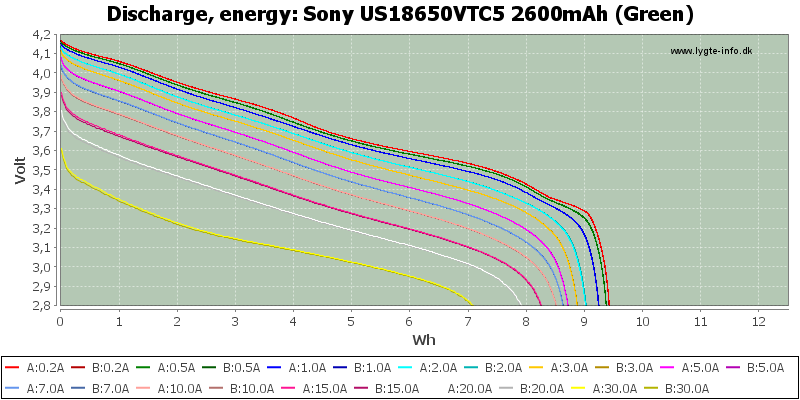
\includegraphics[scale=0.6]{pictures/vtc5.png}
	\caption{Discharge voltage vs. energy for Sony US18650VTC5 cells \cite{vtc5}}
	\label{fig:vtc5}
\end{figure}

\chapter{Balancing test}
\begin{figure}[h]
	\centering
	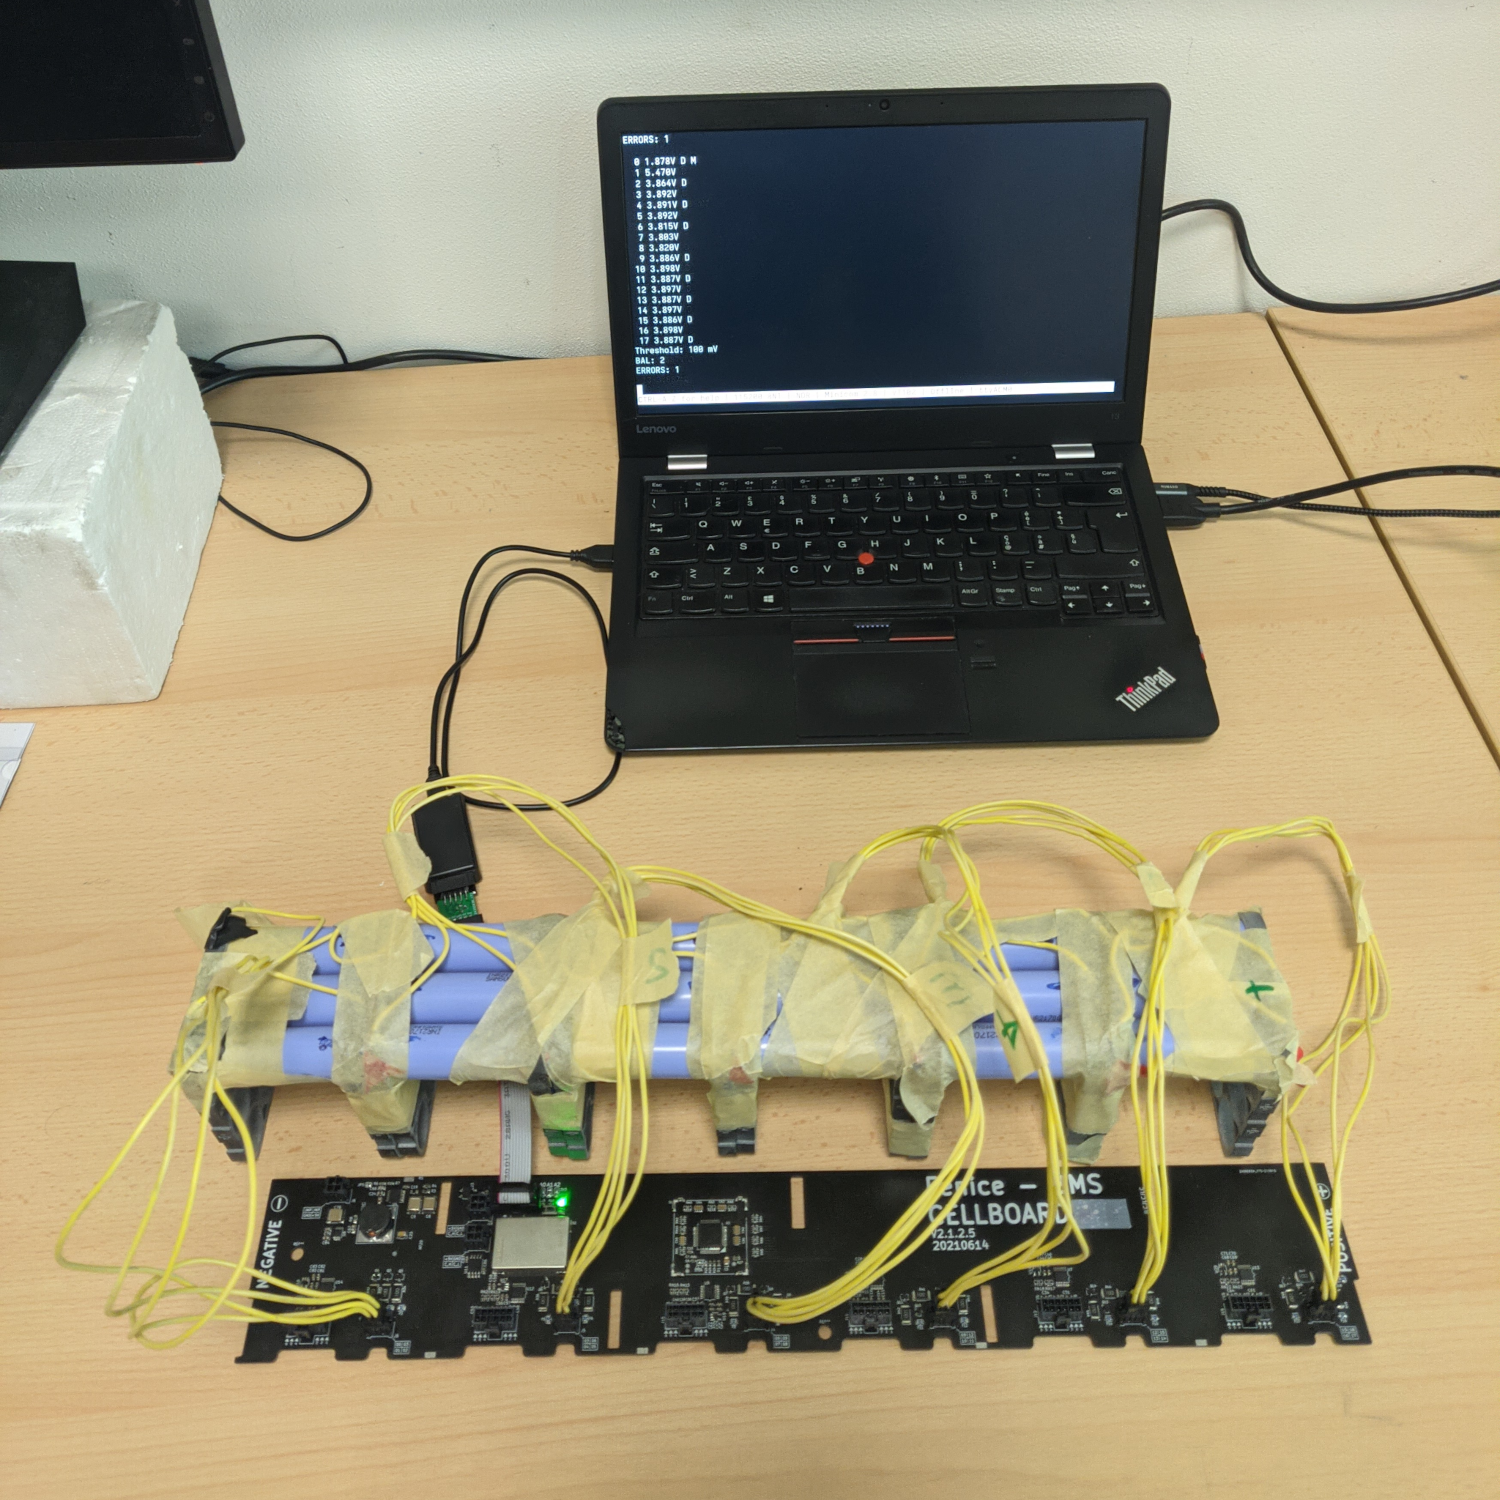
\includegraphics[scale=0.25]{balancing_test.png}
	\caption{Cell balancing test setup.}
	\label{fig:balancing_test}
\end{figure}
\begin{figure}[h]
	\centering
	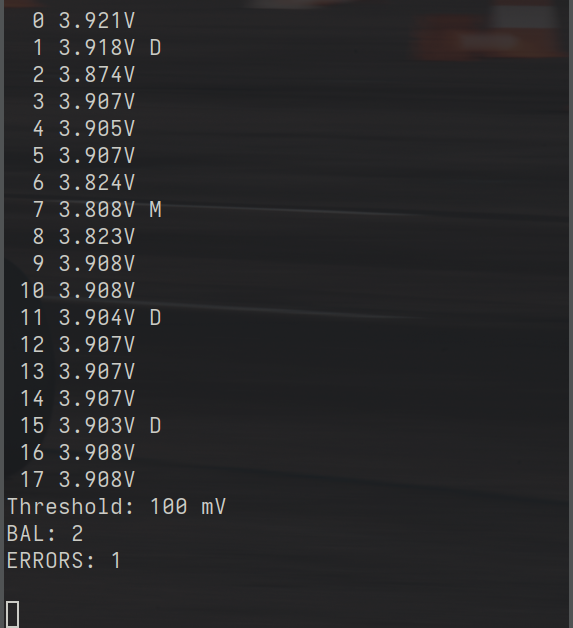
\includegraphics[scale=0.5]{balancing_console}
	\caption{Serial console during balancing. \texttt{M} indicates the minimum voltage, cells marked with \texttt{D} are being discharged}
	\label{fig:balancing_console}
\end{figure}

\chapter{Error management test}
\begin{figure}[h]
	\centering
	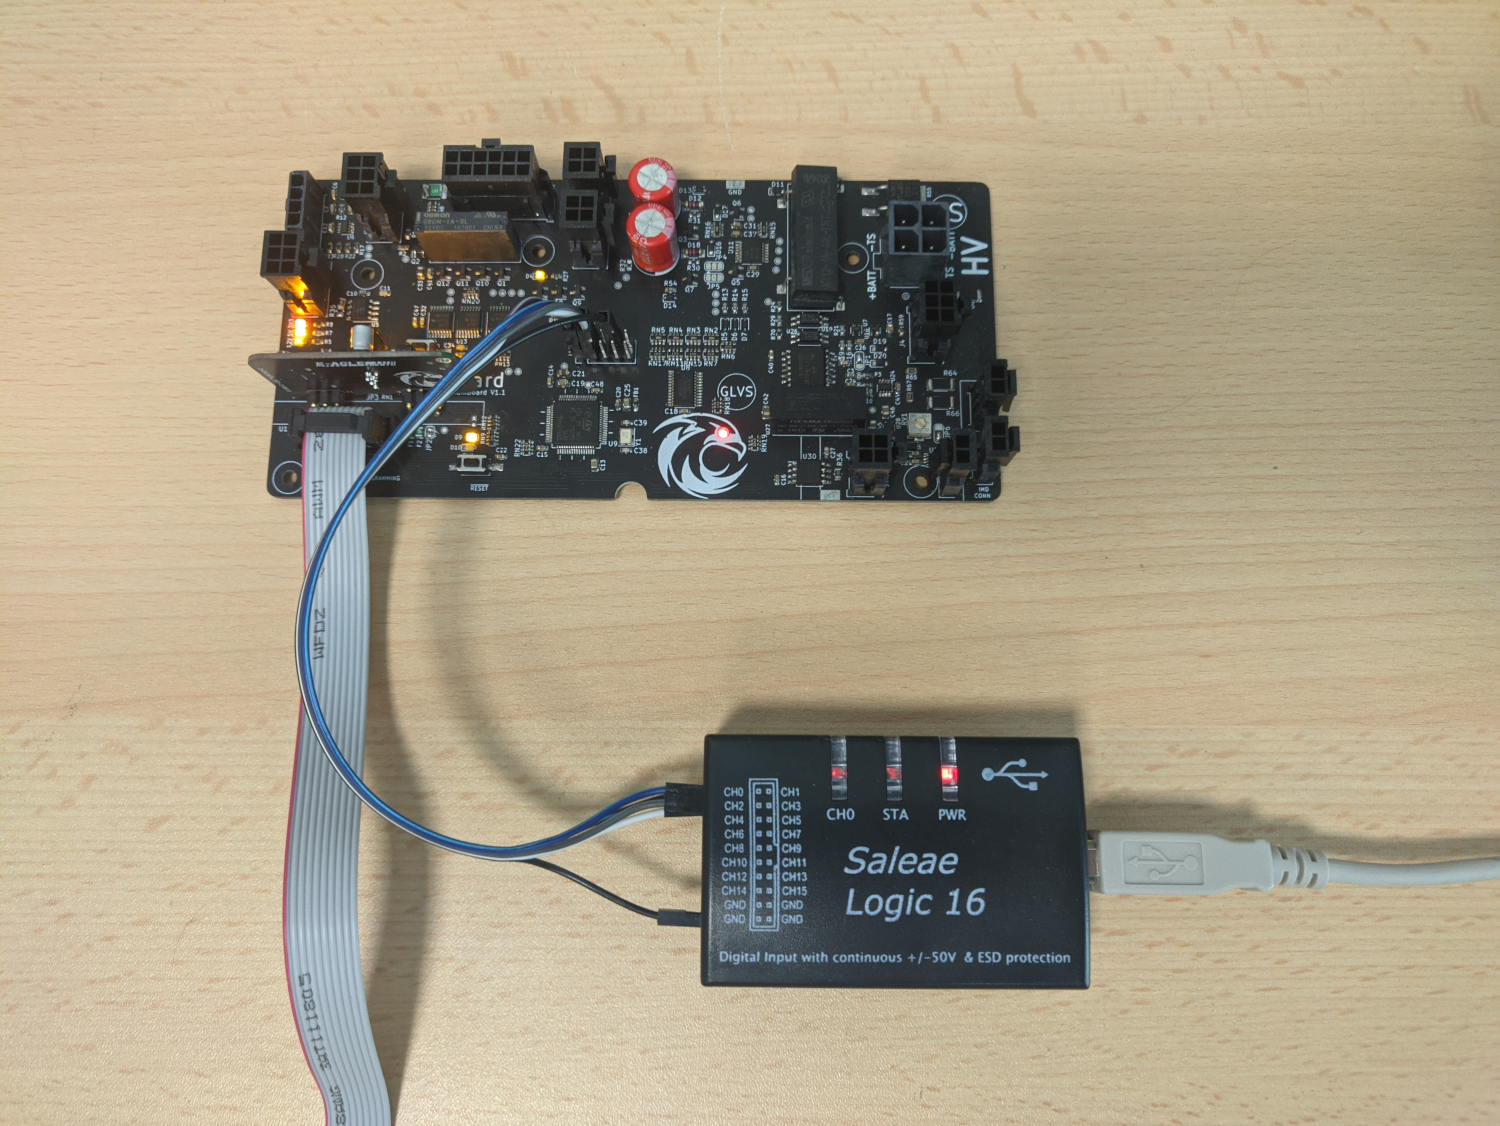
\includegraphics[scale=0.27]{error_test_setup.png}
	\caption{Error test setup with the mainboard and a logic analyzer.}
	\label{fig:error_test_setup}
\end{figure}
\begin{figure}[h]
	\centering
	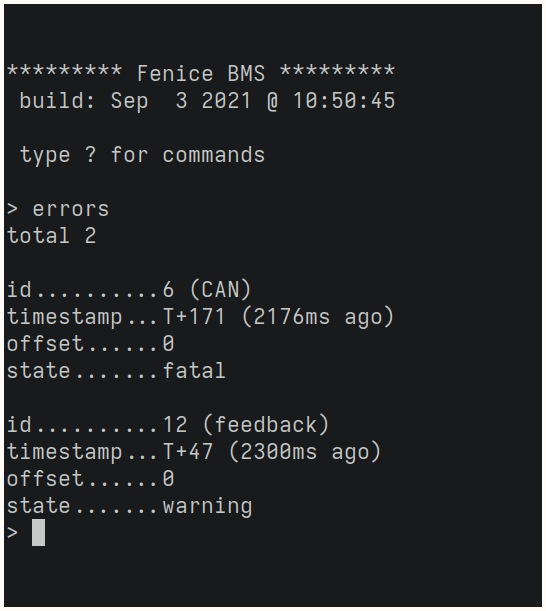
\includegraphics[scale=0.5]{error_console}
	\caption{Serial console reporting active errors.}
	\label{fig:error_console}
\end{figure}